%  \input{header_link}
%   \begin{document}
     		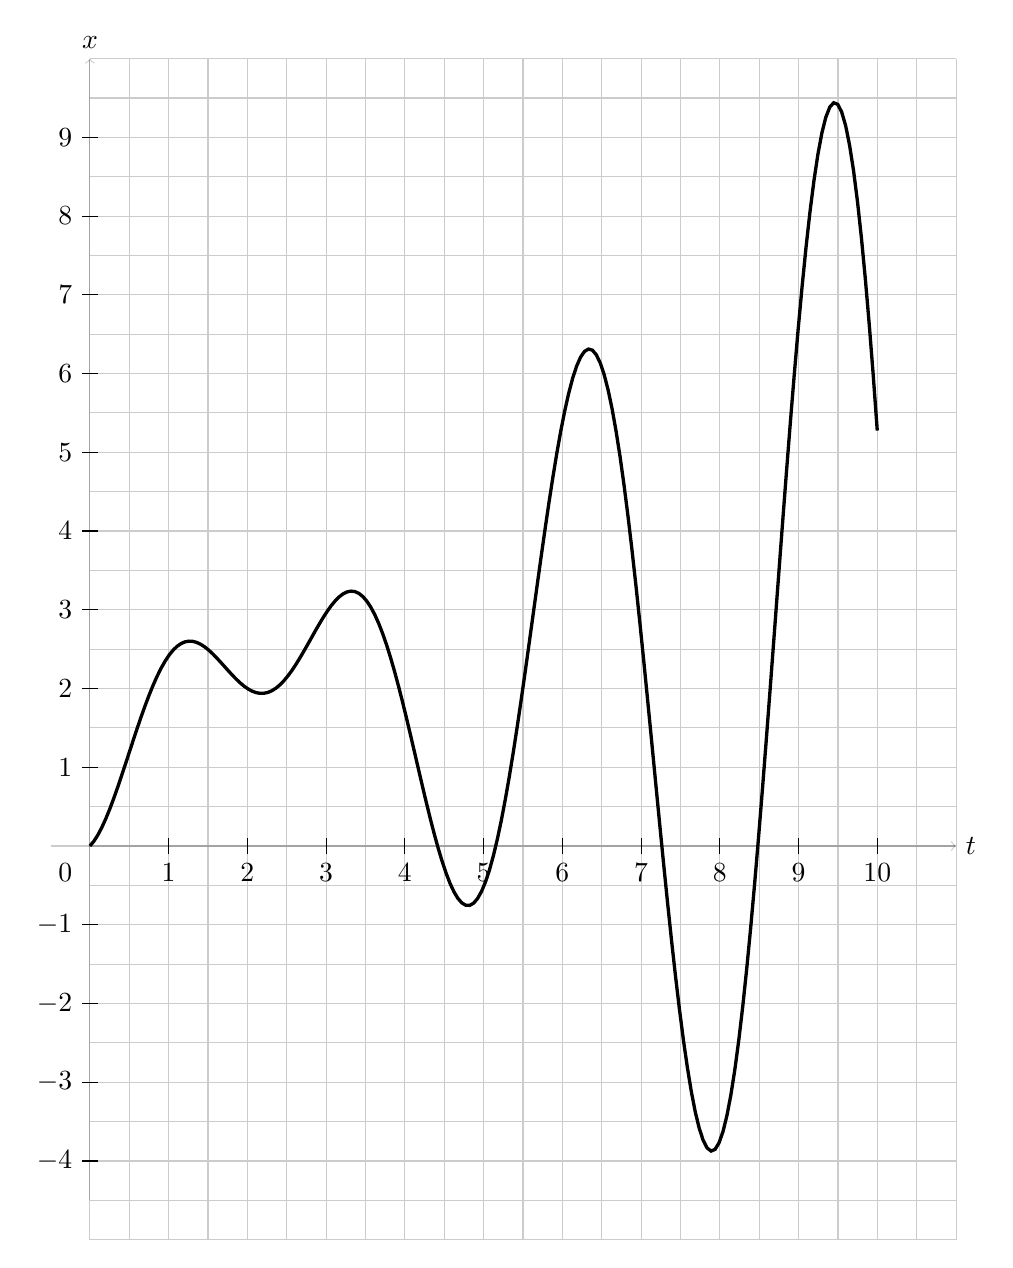
\begin{tikzpicture}[scale=1]
     		\draw[->,opacity=0.2] (-0.5,0)--(11,0);
     		\node[right] at (11,0){$t$};
     		\draw[->,opacity=0.2] (0,-4.5)--(0,10); \node[above] at (0,10) {$x$};
     		\foreach \x in {1,2,...,10}{
     		\draw (\x,0.1)--(\x,-0.1)
     		node[below] {$\x$};}
     		\foreach \y in {-4,-3,...,-1}{
     		\draw (0.1,\y)--(-0.1,\y) node[left]{$ \y$};
     		}
     		\foreach \y in {1,2,...,9}{
     		\draw (0.1,\y)--(-0.1,\y) node[left]{$ \y$};
     		}
     		\node[below left] at (-0.1,-0.1) {$0$};
     		\draw[opacity=0.2,step=0.5] (0,10) grid (11,-5);
            \draw[variable=\t,domain=0:10,samples=200,color=black,line width=1.2pt] plot ({\t},{(\t-2)* cos((2*\t) r)+2});
		\end{tikzpicture}
%  \end{document}
